%\lstinputlisting[language=Matlab]{Cap_4/Es_9/Es_9.m}

%\begin{figure}[H]
%	\label{Cap_4_Es_9}
%	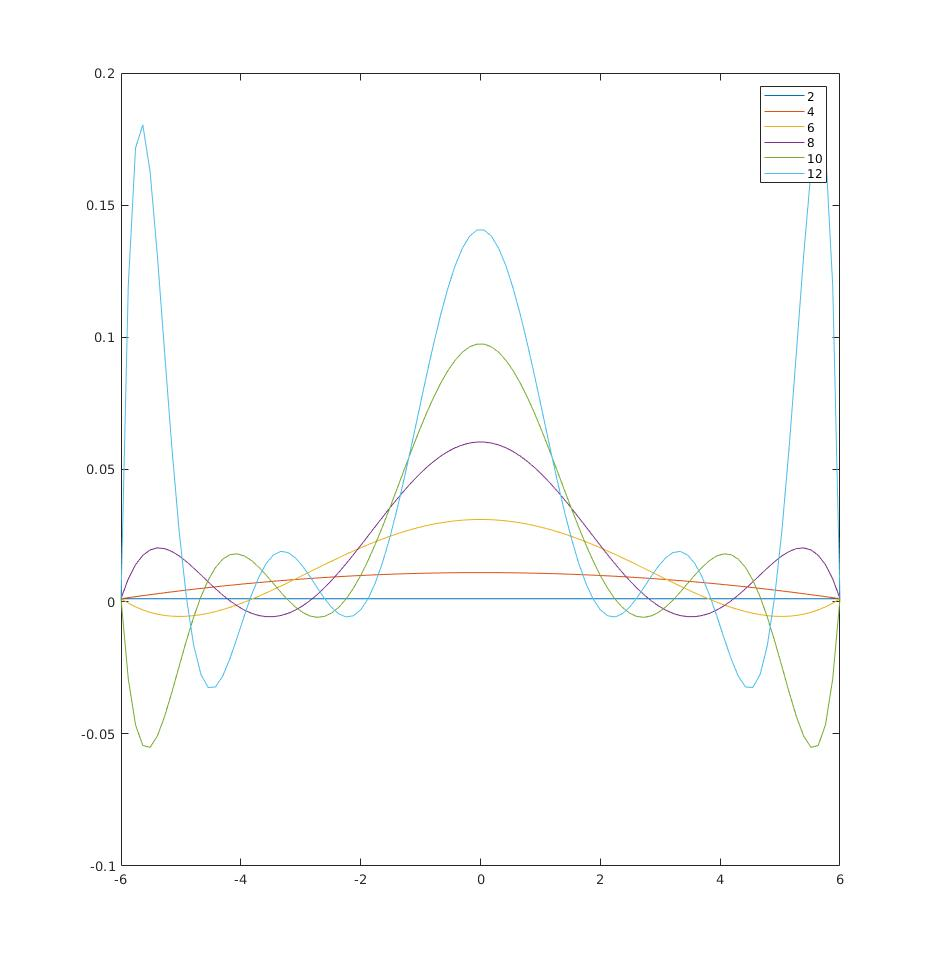
\includegraphics[width=\textwidth]{Plot/Cap_4_Es_9}
%	\caption{Polinomio di Lagrange con n° di ascisse $[2,4,6,8,10,12]$}
%\end{figure}

%\begin{figure}[H]
%	\label{Cap_4_Es_9(1)}
%	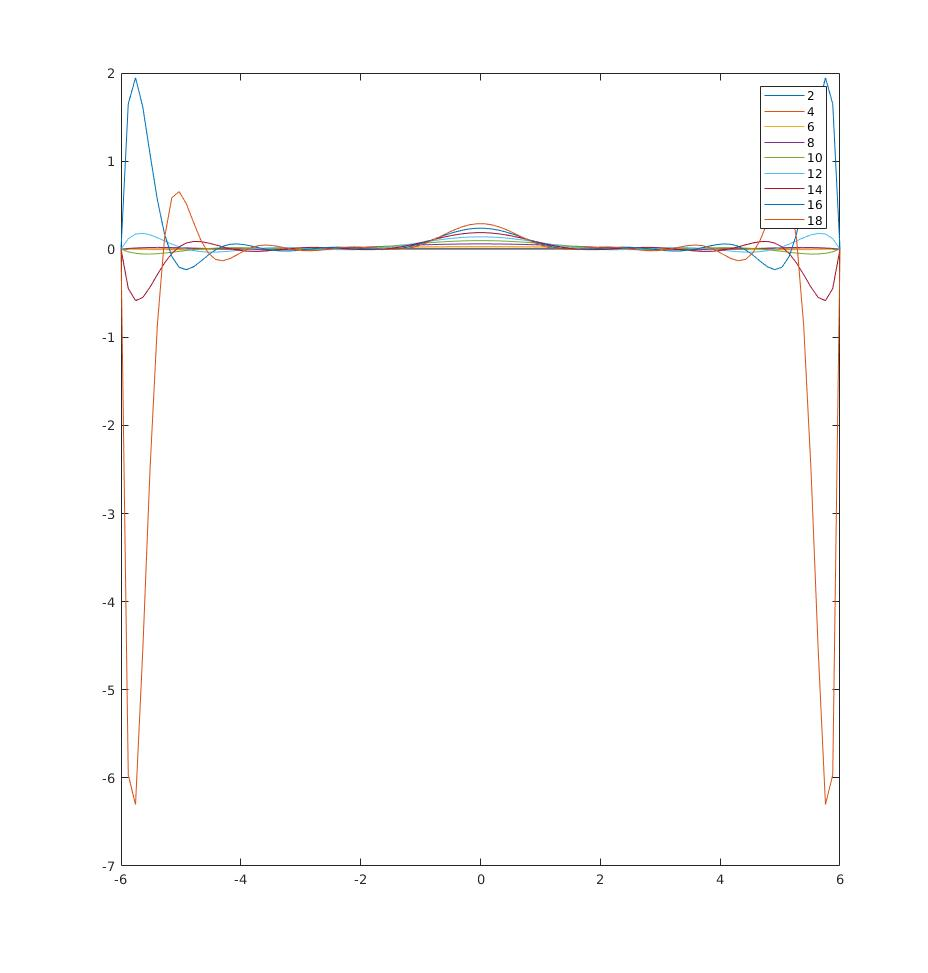
\includegraphics[width=\textwidth]{Plot/Cap_4_Es_9(1)}
%	\caption{Polinomio di Lagrange con n° di ascisse $[2,4,6,8,10,12,14,16,18]$}
%\end{figure}

%\begin{figure}[H]
%	\label{Cap_4_Es_9(2)}
%	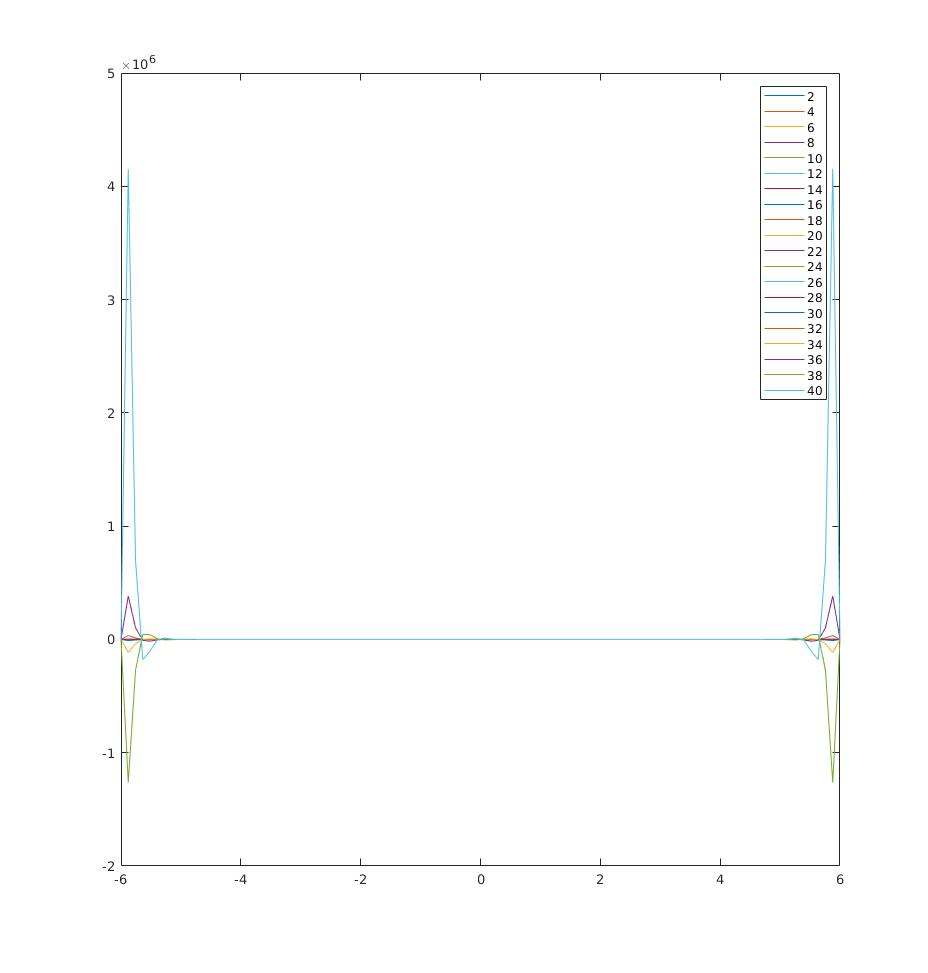
\includegraphics[width=\textwidth]{Plot/Cap_4_Es_9(2)}
%	\caption{Polinomio di Lagrange con n° di ascisse $[2,4,6,8,..,40]$}
%\end{figure}